\begin{definition}[Pullback \cite{pierce1991basic}]
    \label{def:cat:pb}
    \ \newline
\noindent
\begin{minipage}{0.7\textwidth}  
   A \textbf{pullback} of a cospan \(B \overset{\beta'}{\rightarrow} D \overset{\alpha'}{\leftarrow} C \), as shown on the right, is defined as a span \( B \overset{\alpha}{\leftarrow} A \overset{\beta}{\rightarrow} C \) such that \( \alpha \star \beta' = \beta \star \alpha' \), and for every span \( B \overset{\gamma'}{\leftarrow} E \overset{\gamma}{\rightarrow} C \) if \(\gamma' \star \beta' = \gamma \star \alpha'\) holds, then there exists a unique morphism \(\delta: E \to A\) such that $\gamma' = \delta \star \alpha$ and $\gamma = \delta \star \beta$. 
\end{minipage}
\hfill
\begin{minipage}{0.299\textwidth}
    \hfill
\resizebox{0.9\textwidth}{!}{
            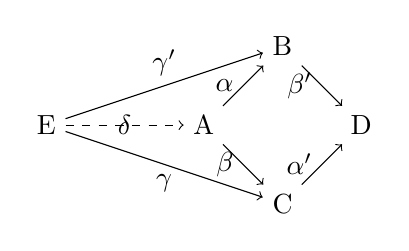
\begin{tikzpicture}
                \node (i) at (0,0) {A};
                \node (r) at (1,1) {B};
                \node (c) at (1,-1) {C};
                \node (h) at (2,0) {D};
                % \node () at (1,-1) {\( \Delta \)};
                \draw[->]  (i) -- (r) node [midway,left] {$\alpha$};
                \draw[->] (c) -- (h) node [midway,left] {$\alpha'$};
                \draw[->] (r) -- (h) node[midway, left] {$\beta'$};
                \draw[->] (i) -- (c) node[midway, left] {$\beta$};
                \node (d') at (-2,0) {E};
                \draw[<-] (c) -- (d') node [midway,below]{$\gamma$};
                \draw[<-] (r) -- (d') node [midway,above]{$\gamma'$};
                \draw[->, dashed] (d') -- (i) node [midway]{$\delta$};
            \end{tikzpicture}
}
\end{minipage}
The diagram involving \(\alpha\), \(\beta\), \(\alpha'\), and \(\beta'\) is referred to as the \textbf{pullback square}, \(A\) as the \textbf{pullback object}, and the existence of the unique morphism is known as the \textbf{universal mapping property of the pullback}.
\end{definition} 